%%%%%%%%%%%%%%%%%%%%%%%%%%%%%% -*- Mode: Latex -*- %%%%%%%%%%%%%%%%%%%%%%%%%%%%
%% 09-07.tex --      IEEE Service Cup Paper
%% Author          : Philip Johnson
%% Created On      : Mon Sep 23 11:52:28 2002
%% Last Modified By: Philip Johnson
%% Last Modified On: Thu Feb 12 13:49:01 2009
%%%%%%%%%%%%%%%%%%%%%%%%%%%%%%%%%%%%%%%%%%%%%%%%%%%%%%%%%%%%%%%%%%%%%%%%%%%%%%%
%%   Copyright (C) 2009 Philip Johnson
%%%%%%%%%%%%%%%%%%%%%%%%%%%%%%%%%%%%%%%%%%%%%%%%%%%%%%%%%%%%%%%%%%%%%%%%%%%%%%%
%% 

%% Home page: http://iscc.servicescomputing.org/2009/
%% We are applying to the ``Service Computing Contest'' (for university professors/projects)

%% Should show how Hackystat explores ``new frontiers'' in SOA development.
%% 8 page limit for paper.
%% At most five students plus one professor.
%% Due date: February 20, 2009.  
%% Conference: July 7-10, 2009, Los Angeles.

%% Paper ID: 1122, http://confhub.com/MyPapers.php?cid=66

%% For ``peer review mode'', do:
%%   \documentclass[conference,compsoc,peerreview]{IEEEtran}
%% and
%%   \IEEEpeerreviewmaketitle  (after the abstract).

%\documentclass[conference,compsoc,peerreview]{IEEEtran}
\documentclass[conference,compsoc]{IEEEtran}
\usepackage[final]{graphicx}
\usepackage{cite}
\usepackage{url}
% uncomment the % away on next line to produce the final camera-ready version
% and uncomment the \thispagestyle{empty} following \maketitle
%\pagestyle{empty}

\begin{document}

\title{Experiences with Hackystat \\ as a service-oriented architecture}

\author{Philip M. Johnson \\
        Shaoxuan Zhang \\
        Pavel Senin \\
\em  Collaborative Software Development Laboratory \\
      Department of Information and Computer Sciences \\
      University of Hawai'i \\
      Honolulu, HI 96822 \\
      johnson@hawaii.edu \\
}


\maketitle
%\IEEEpeerreviewmaketitle
%\thispagestyle{empty}

\begin{abstract}  % 200 words
Hackystat is an open source framework for automated collection and analysis
of software engineering process and product data.  Hackystat has been in
development since 2001, and has gone through eight major architectural
revisions during that time.  In 2007, we performed the latest architectural
revision, whose primary goal was to reimplement Hackystat as a
service-oriented architecture (SOA).  This version has now been in
public release for a year, and this paper reports on our experiences:
the motivations that led us to reimplement the system as a SOA, the
costs and benefits of that conversion, and our lessons learned. 
\end{abstract}


\section{Introduction}
\label{sec:intro}

Software engineering measurement is a compelling practice in principle. By
gathering data on the structure and quality of code, as well as the
behaviors of the developers as they build it, one can imagine obtaining
useful insight into the current state of development, better estimates of
what lies in store for the future, and ideas on how to improve current
practices and work artifacts.

The reality is that software engineering measurements are difficult to
obtain and difficult to interpret. To the extent that measurements are made
manually, this incurs overhead on the development staff which might seem
expendible when the schedule is tight.  Even if measurements are made,
useful insight and action is often difficult to obtain.  Is test case coverage of 70\%
good, bad, or someplace in between? Even if everyone agrees it is bad, what
exactly should be done, if anything?

Since 2001, we have been developing an open source framework for automated
collection and analysis of software engineering process and product data
called Hackystat (\url{http://www.hackystat.org/})
\cite{csdl2-06-06,csdl2-02-07}.  The goal of Hackystat is to provide an
extensible mechanism that can radically reduce the overhead associated with
collection of a wide variety of software engineering data, along with a
sophisticated toolkit of analyses that can facilitate useful
interpretation.  Over the years, Hackystat has been used in a wide variety
of application areas, including: classroom pedagogy,
inference of test-driven design practice, software
engineering of high performance computing systems, and a
telemetry-based approach to software measurement trend definition and
display.

The Hackystat Framework is intended to be generic: it strives to be neutral
with respect to the platform, programming language and environment,
development process, and application domain.  We have not found this to be
a simple goal, and the architecture of Hackystat has undergone eight
significant revisions since 2001 in response to new application demands
upon the framework.

One of the most significant architectural revisions is the most
recent one, which occurred in 2007 when we migrated the Hackystat Framework
from a traditional client-server web application architecture to a
service-oriented architecture (SOA) using REST design principles.  This
required eight months of development and a rewrite of most of the system
(which by that time had grown to approximately 350,000 lines of code).

There are several reasons why we believe Hackystat is an interesting
example of a service oriented architecture.  First, it is a mature and
non-trivial system whose entire source code history is available and whose
conversion to SOA was motivated by concrete design issues.  Second, it
appears to be the first and only SOA-based software engineering data
collection and analysis system.  Other such systems (including SixthSense
Analytics, Programeter, Devcreek, SonarSource, ElectroCodeoGram, and EPM)
all have a client-server architecture.  Finally, Hackystat implements a
carefully designed combination of distributed computation, caching, and
pre-fetching that attempts to provide the flexibility and scalability of
SOA without sacrificing the performance of a simpler client-server
architecture.

The SOA version of Hackystat has been in public release for approximately
one year, and this has given us sufficient time to start to understand the
changes, both positive and negative, that have resulted from this move.
Section \ref{sec:motivation} discusses the shortcomings of our prior
Hackystat architecture which led us to reimplement the system in a
service-oriented manner.  Section \ref{sec:soa} introduces our current
service-oriented architecture and its features.  Section
\ref{sec:discussion} presents our experiences, both positive and negative,
with the SOA implementation.  Section \ref{sec:conclusion} summarizes our
lessons learned.


\section{Motivation for the Hackystat SOA architecture}
\label{sec:motivation}


\begin{figure*}[ht]
  \center
  \includegraphics[width=0.7\textwidth]{configurations5.eps}
  \caption{Two example Version 7 configurations}
  \label{fig:configurations}
\end{figure*} 

Hackystat architectural design decisions has always followed an ``agile''
approach of implementing ``the simplest thing that could possibly work''.
Since 2001, this has resulted in eight significant re-designs of the system
as it outgrew the constraints imposed by the previous architecture.  Some
might view this as a process-level bug, but we view it as a feature: we
could never have predicted in advance which application areas Hackystat
would be used in and the specific architectural pressures they would
create.  As a result, Hackystat's current implementation as a SOA
architecture is not based upon SOA being the current ``hot'' architecture,
but rather as a response to specific issues we were facing with the
previous version and the hope that SOA could address them.

To understand the costs and benefits of Hackystat Version 8, it is
important to know a little bit about its predecessor, Version 7.  First, by
the time of Version 7, Hackystat had grown to support software engineering data
collection and analysis in a variety of very different domains, including
Java-based classroom instruction, C-based high performance computing, Java
and Visual Studio-based test driven design inference, build system analysis
for NASA, a ``continuous'' approach to the Goal-Question-Metric paradigm,
and others.  To support sharing of overlapping functionality between these
domains, the 350 KLOC in the system were broken down into approximately 70
different modules.  While it was possible to build a release of Hackystat
containing all of these modules (and we did so for testing purposes), we
found that any particular domain of application was much better served by
supporting Hackystat ``configurations'', or builds of the system containing
a subset of all possible modules.

Figure \ref{fig:configurations} illustrates Hackystat modules, subsystems,
and configurations in Version 7.  It shows samples of modules (such as
``Standard'', ``HPC Experiment'', etc.) from two configurations: HPC and
Classroom.  Although only 10 modules are shown in the figure due to space
limitations, Hackystat 7 configurations typically contained from 30 to 60
modules.


Modules were assigned to one of four ``subsystems'' depending upon their
functionality: the ``Sensor'' subsystem contains modules providing software
``plugins'' to various tools; the ``SDT'' subsystem contains
implementations of structured sensor data called``sensor data types'', the
``Core'' subsystem provides basic client and server-side infrastructure,
and the ``App'' subsystem contains domain-specific analyses and user
interface facilities.


Each module in Hackystat was managed as a separate Subversion project, but
most could not be compiled individually. Instead, the build process would
take in a description of a Hackystat configuration as a list of modules,
and then compile those modules together into a functional client-server
application and run the set of tests associated with the included modules.
Each Hackystat module was required to indicate the other modules that it
depended upon so that the build process could sequentialize and resolve
dependencies.  If, during the build of a configuration, the system
encountered a module with a dependency that was not included in the
configuration list, an error was signalled.

Let's now turn to some of the problems we encountered with this approach to
modularity and flexibility within the confines of a client-server
architecture.

\subsection{System configuration binding time}

In the Version 7 architecture, we defined a system configuration as a list
of modules and then invoked the build system to produce a binary containing
those sets of modules.  This approach was the most straightforward way to
build a single client-server system with a subset of all possible modules
while still enabling testing and dependency resolution.

It did mean, however, that any user wanting to create a new configuration
adapted to their specialized needs would have to learn how to build the
system from sources. In Version 7, one could not take an existing binary
release and augment its functionality without recompilation. 

\subsection{Complexity of build}

We discovered that our need for a configurable system building process
exceeded the standard capabilities of Ant, the canonical Java build system
tool.  To resolve this, we created a custom Hackystat build system
``wrapper'' around Ant.  This wrapper would take as input an XML
description of a Hackystat module and its dependencies, and generate a
number of Ant scripts that would correctly order the sequence of targets
for a particular configuration.

While the build system wrapper worked quite well, and actually automated
the generation of many thousands of lines of Ant build scripts, the problem
was that new Hackystat developers now needed to learn a custom 
system in order to build Hackystat.  Furthermore,
not only developers of new Hackystat modules needed to learn this build
system, but even those who simply wanted to create a custom configuration
from existing modules needed to learn it.


\subsection{Lack of access to ``intermediate'' analyses}

In the early stages of Hackystat development, sensor data was sent to a web
server, which performed relatively simple analyses over that data before
presenting that data to the user in a web page.  As the complexity of our
analyses increased, we found it useful to decompose some of them into
pipelines of smaller analyses.  For example, to obtain telemetry (trend)
data, the raw sensor data would first be analyzed into intermediate objects
called ``DailyProjectData'', which would then be input into the Telemetry
mechanism and further refined to produce the trends of interest.  As a
second example, the Test-Driven Design analysis would first organize the
raw sensor data into ``episodes'' which would then be input into a
rule-based system for classification with respect to TDD compliance.

Figure \ref{fig:subsystems} illustrates this aspect of the internal structure
of the server.  Raw sensor data ``percolates up'' through a series of analyses
to form increasingly higher level abstractions.  Some intermediate analyses 
(such as the SensorData analysis) could be used by multiple higher level analyses.

\begin{figure}[ht]
  \center
  \includegraphics{subsystems.eps}
  \caption{Version 7 subsystems and pipelines}
  \label{fig:subsystems}
\end{figure} 

One resulting problem with this pipeline is that though the intermediate
results were often interesting in their own right, they were not easily
accessed outside of the server-side processing mechanisms. Another problem 
resulted from caching, as discussed below in Section \ref{sec:caching}.

\subsection{Server-side and build language specificity}

The Hackystat framework is designed to be generic within the domain of
collection and analysis of software engineering process and product data.
It should run on all platforms, support sensors for arbitrary software
development tools and languages, and support analyses for a wide variety of
process and product measurement types.

The same language ``neutrality'' did not hold true when it came to the
framework itself.  Client-side sensors could (and were) written in a
variety of languages: Java, C\#, Emacs Lisp, etc. The server, however, was
a Java web application, and all analyses and user interfaces were required
to be written in Java and conform to the Hackystat web interface structure.

Similarly, the build system for Hackystat Version 7 was Ant, and the only
supported container for the server web application was Tomcat.

\subsection{UI rigidity}

To simplify UI development, Version 7 provided a high-level API for adding
new commands to the Hackystat web application interface which provided a
very standard look and feel.  Figure \ref{fig:commands} illustrates two
commands from Version 7 and their standardized look-and-feel.

\begin{figure*}[ht]
  \center
  \includegraphics[width=0.7\textwidth]{v7commands.eps}
  \caption{Two example Version 7 commands illustrating the common look and feel}
  \label{fig:commands}
\end{figure*} 

When first implemented, the user interface API saved time.  Though there
was a learning curve associated with it, the API enabled the set of modules
in a given configuration could contribute its own set of commands to the
user interface.  It also guaranteed that all commands would exhibit the
same user interface. Finally, we implemented an API that made it simple to
programmatically invoke commands in the user interface from test code.

By the time of Version 8, we began to feel that the user interface standard
was also a straightjacket: Hackystat's architecture was effectively
``frozen'' with a single user interface style and both the build system and
test system (as well as actual UI code) would need to be changed
significantly in order to support experimentation with alternative user
interfaces.

\subsection{Cache thrash}
\label{sec:caching}

In the Telemetry application, it was not uncommon to regularly request an
analysis that might display 30 or 40 trend lines for a set of software
projects over the last several months. Such a request could easily involve
the processing of hundreds of thousands of raw sensor data
instances. However, many of those trend lines might require access to the
raw same sensor data, and many if not most of the trend line components
might involve computations that were performed previously the last time the
analysis was requested.

We quickly discovered that a naive implementation of telemetry could
easily take several hours to perform common types of analysis, but that our 
``pipeline'' approach to analysis lent itself naturally to caching.

The basic idea is simple: use caches to store the results of intermediate
computations.  Referring again to Figure \ref{fig:subsystems}, we
implemented a cache for Sensor Data (which avoided to cost of going to the
database), a cache for Daily Project Data instances (which avoided the cost
of re-processing Sensor Data), and a cache for Episodes (which again
avoided the cost of re-processing Sensor Data).

The introduction of multiple caches worked extremely well for a while.
Computations which could have taken hours now took only seconds or minutes.
Unfortunately as the system continued to grow in size and complexity,
caching began to create problems of its own.  The millions of sensor data
instances in a Hackystat sensor data repository meant that we could not
simply cache everything; we needed to limit the size of the various caches.
As the number of caches for different types of intermediate objects
increased, we started to see evidence of ``cache thrash'': one cache
appeared to be discarding objects just as another cache would be requesting
them. Tuning the various caches to maintain the right size and work
effectively with each other constituted a difficult performance analysis problem.

\section{Hackystat as SOA}
\label{sec:soa}

To summarize, Hackystat's original client-server architecture worked well
when Hackystat processed relatively few kinds of data in relatively few
kinds of ways for a relatively small number of users.  We hypothesize that
the prior architecture would have scaled well, at least for a while, if
growth had been restricted to just one of these three dimensions.

Unfortunately, the system grew in scale along all three of these dimensions
simultaneously.  We attempted to manage its size and complexity while
staying within the basic client-server architectural model in several ways:
by a custom module system to support configurations; by pipelining analysis
processing; by caching; and by high level APIs for the user interface,
build system, and testing.

By 2007, however, we realized that we had designed ourselves into a
corner: the system structure was well suited to a certain performance
load and set of application domains, but the features that achieved that
also actively prevented us from other kinds of extensions and enhancements.

After a month of discussion, we halted all development on the Version 7
code base and started over with a new architectural paradigm: a RESTful
service-oriented architecture.  Figure \ref{fig:soa} illustrates some of 
the services now available or in active development in Version 8.

\begin{figure*}[ht]
  \center
  \includegraphics[width=0.7\textwidth]{soa.eps}
  \caption{Services now available or in development for Hackystat Version 8}
  \label{fig:soa}
\end{figure*} 

A comparison of Figure \ref{fig:soa} with Figure \ref{fig:subsystems}
reveals several of the major similarities and differences between the old
client-server architecture and the new service-oriented architecture.
First, Hackystat Version 8 retains a similar kind of pipelined, incremental
approach to analysis that was present in Version 7. This is illustrated by
the presence of uniformly upward pointing arrows in both Figures.  In both
versions, raw sensor data is stored in a database and ``percolates upward''
through various kinds of analyses toward a user interface.

However, in Version 8 there is no longer a ``box'' around the analyses,
indicating that instead of a single server, Hackystat now consists of a
number of cooperating services, some of which correspond relatively
directly to analysis subsystems within the old system (such as SensorBase,
DailyProjectData, and Telemetry), and others of which are brand new:
ProjectBrowser, Tickertape, and TrajectoryViewer.

In Figure \ref{fig:subsystems}, the arrows essentially correspond to Java
method invocations all within a single process.  In Figure \ref{fig:soa},
the arrows correspond to HTTP calls designed according to REST
(Representational State Transfer) principles \cite{Fielding02}.

\section{Pros and cons of SOA}
\label{sec:discussion}

The re-implementation of Hackystat as a service-oriented architecture was
not trivial: it required eight months of effort, and we have still not
completed the porting of all the capabilities present in Version 7.  

On the other hand, the move to a service-oriented architecture has broken
the ``design knot'' that we found ourselves in with Version 7 and has
enabled us to explore new interfaces and capabilities that were effectively
precluded by the old architecture.  

As part of the move to Version 8, we also moved to Google Project Hosting.
Each service in Hackystat 8 is managed as an independent project.  There
are currently over 40 separate projects related to Hackystat at Google
Project Hosting. 

Let's begin the analysis of the pros
and cons of SOA for our domain by revisiting the issues we confronted in
Version 7 as described above:

\subsection{Server-side and build language specificity}

One of the fundamental benefits of moving to a SOA architecture has been
the elimination of Java and Ant as the required server-side implementation
language and build tool.  In Version 8, each service is developed as an
independent project (normally hosted at Google Project Hosting, although
even this is not mandatory).  Because each service communicates with each
other via HTTP, the only constraint on language choice is the ability to
process the HTTP networking protocol; a feature available in all modern
programming languages.  In addition to Java, services have been already
been developed using Perl, Python, and Flex.  A service implementation is
similarly free to choose the most appropriate build tool for its
environment.

%% \subsection{System configuration binding time}

%% In Version 7, a Hackystat configuration was defined at compile time, which
%% meant that users needed to understand the build system in order to create
%% new configurations or augment an existing configuration with a new feature.
%% In Version 8, system configurations are defined at run time based upon what
%% set of services a site administrator chooses to invoke.  

%% Pro: Restart a single service without bringing down entire system.

%% Con: Loss of compile-time structural consistency checking for sensor data types.


\subsection{Complexity of build}

Version 7 required a custom build system which created a barrier to entry
for new developers.  This problem no longer exists, as each service in
Version 8 can choose its own language and build technology.

\subsection{Lack of access to ``intermediate'' analyses}

Another substantial benefit of the SOA architecture is the ``opening up''
of the analysis pipelines that were formerly embedded within the Version 7
client-server architecture.

In Version 8, major analysis components, such as the raw sensor data, daily
project data, and telemetry have been encapsulated within their own
individual services.  This open architecture means that all stages of an
analysis pipeline are now accessable for extension and reuse. 

\subsection{UI rigidity}

Any client-server architecture implicitly requires a choice of a single
user interface technilogy: be it Java, Ruby on Rails, PHP, etc.  By moving
to a service-oriented architecture, we freed ourselves from having to make
this choice. Hackystat is now able to support many different user
interfaces, including both web-based (via a browser) or client-side
(native).  This has facilitated entirely new avenues for research and
development, including advanced 3D visualization (requiring a native client
user interface) and integration with social networking user interfaces such
as Facebook and Twitter.  Figure \ref{fig:icu} illustrates one such 
interface made possible by Version 8 called the ``Software ICU'' which uses 
layout, color, sparklines, and sortable columns in a way not possible in Version 7:

\begin{figure*}[ht]
  \center
  \includegraphics[width=1.0\textwidth]{icu.eps}
  \caption{The Software ICU interface, made possible by Version 8}
  \label{fig:icu}
\end{figure*} 

\subsection{Cache thrash}
\label{sec:v8cache}

There is one spectacular downside in the move from client-server to SOA
architecture: what was once an in-memory method invocation (i.e. the arrows
in Figure \ref{fig:subsystems} is now an HTTP request (i.e. the arrows in
Figure \ref{fig:soa}).  In-memory object retrievals that took less than a
millisecond in Version 7 could now require at least one HTTP request
requiring 20 to 100 milliseconds or more.  This constitutes a two to three
order of magnitude performance hit!  Note that the more ``arrows'' that must be traversed 
to perform an analysis, the worse the potential performance hit becomes. 

As a simple yet realistic example of the problem, the Software ICU
interface shown in Figure \ref{fig:icu} illustrates current values and
trends for nine metrics on five projects, each with around 5 developers,
over five weeks. Without caching, each trend requires one HTTP request from
the telemetry service, for a total of 9 trends/project * 5 projects = 45
HTTP requests.  To build each trend line, the Telemetry service must ask
for at least one DailyProjectData instance per day, or 7 days/week * 5
weeks = 35 HTTP DailyProjectData requests per trend line.  Since we have 45
trends to compute, that's 35 HTTP requests / trend * 45 trends = 1575 HTTP
requests.  Now it gets really bad, because the computation of a single
DailyProjectData request could easily require the processing of 100
SensorData instances on average.  This brings the total number of HTTP
requests to 1575 * 100, or 157,500 HTTP requests in order to build the
Software ICU visualization.  If we are optimistic and assume an average
HTTP request/response cycle requires only 20 ms, that means the
communication overhead alone for this request is almost an hour, without
adding in the actual computation time!

The ``communication'' requirements for a client-server system implementing
the Software ICU would be similar, except that instead of 157,500 HTTP
requests, a client-server system would require 157,500 method invocations.
Assuming a method invocation takes 1 ms, the communication requirements
drop to a little over 2 minutes.

This is not a simple problem to resolve, and the Hackystat development
community has so far initiated two different approaches to dealing with
it.

First, we have implemented URL caches in certain intermediate services such
as Daily Project Data and Telemetry.  One of the benefits of a RESTful API
design is the ability to exploit well understood HTTP caching and cache
control mechanisms.  A characteristic of Hackystat's domain is that
historical analysis data instances rarely change once they have been
computed, making them extremely well suited to caching.  We built a generic
cache facility based upon Apache JCS (Java Caching System) which supports
very fast disk-backed mapping of URLs to the associated response
object. These caches eliminate a significant amount of computation as well
as HTTP requests.  For example, if a developer requests the Software ICU
visualization once a week, then four out of the five weeks of trend data
will be cached from previous invocations, resulting in an 80\% reduction in
HTTP communication overhead.

This is good, but we can do even better via a mechanism we designed called
``prefetching''.  The idea of prefetching is that if you know you'll want
an analysis once a week, then simply set up a timer-based process to
request that analysis once a day, discarding the results.  Prefetching is
quite powerful in several ways.  First, it pre-fills the caches for the
analysis of interest. This means that in the case of our Software ICU
example, the number of HTTP requests is reduced to 45, which typically introduces under a
second of communication overhead.  Second, due to the nature of the
service-oriented architecture, many other related analyses benefit as
well. For example, filling the DailyProjectData cache will speed up all
services requesting that data, not just the Software ICU.  Finally,
repeatedly prefetching introduces much less overhead on the system than one
might expect, because most of the prefetch involves previously cached data
by design.

%% \subsection{Other issues}

%% There are several other interesting results from our move to SOA that are
%% worth a brief mention.

%% First, we have observed no appreciable change in the number of lines of
%% code required to implement a given functionality.  SOA appears to require
%% neither more code nor less code than a client-server equivalent.  However,
%% SOA does require very different code than a client-server system, and
%% Version 8 led us to new libraries (such as Apache JCS and the Restlet
%% framework).

%% Our SOA architecture makes it almost trivial to support certain kinds of
%% scalability.  For example, we can run all services on a single physical
%% host, or distribute each service to a different physical host by simply
%% editing a configuration file.  More interestingly, it is now possible to
%% transparently replicate certain services.  For example, if we find that the
%% telemetry service is a bottle neck in processing, we can simply run two
%% telemetry services and partition requests between them.

%% Finally, it is a common axiom of software engineering that the software
%% architecture tends to reflect the organizational architecture.  Our
%% experience is that the reverse is also true: the move to SOA also has
%% resulted in a significantly more decentralized, non-hierarchical
%% development organization.  In Version 7, the requirement that new
%% functionality had to be written in Java, introduced into our build system,
%% and maintained in our internal code repository created a barrier that only
%% committed Hackystat developers were willing to climb.  In the new
%% architecture, each service is publically available as an individual Google
%% Project, and developers and users can much more easily adapt, extend, and
%% integrate without any interaction from the core Hackystat development team.

\section{Lessons Learned}
\label{sec:conclusion}

After one year of use, we are quite happy with our decision to move to a
service-oriented architecture, though it has not been without
challenges. Here are some of the lessons we learned from our experience.

\subsection{SOA introduces costs}

Our move to SOA was not cheap.  First, forward progress on functionality was
arrested for approximately eight months while we performed an almost
complete reimplementation of the system.  We do not believe that
``retrofitting'' a service-oriented architecture on our prior code base
would have been effective, and ultimately might have taken longer than
simply starting over.  

Second, the move to SOA meant that our developers needed to learn new
architectural concepts (such as REST) as well as new libraries (such as
Apache JCS).  This was part of the reason why the process took so long.

\subsection{SOA decouples on multiple levels}

Our new SOA architecture has decoupled not only our system, but also our
development process and even our organization.  As described above, our
previous architecture enforced a common language (Java), a common build system (Ant
plus custom extensions), and ultimately a common way of doing development (via the
quality assurance mechanisms and standards we implemented).

With SOA, these technological constraints which could be exploited to
enforce ``best practices'' have been removed.  As a simple example, it is
hard for Java programmers to perform effective and useful code reviews on
Python code; we do not have the experience to question, for example,
whether a chosen Python library for XML processing is best suited to the
purpose. Similarly, a Hackystat service choosing a decentralized
configuration management system such as GIT will move toward a much
different style of collaborative development than our traditional,
Subversion-based procedures.  This has organizational implications.

The kind of decoupling introduced by SOA also means that certain kinds of
``bindings'' occur at run-time rather than at build-time or compile-time.
This introduces new complexities into quality assurance, as certain kinds
of inconsistencies are now found only during run-time testing.  Such
problems are made more difficult to catch due to the more decentralized and
distributed nature of development.

\subsection{SOA requires governance}

The novel forms of decoupling introduced by SOA leads to the need for new
kinds of ``governance'' we did not previously require.  For example, one
group of developers embarked on a project to implement a new kind of
low-level service that would effectively ``collapse'' functions spread
across multiple services into a single layer.  This service would improve
performance for certain kinds of queries in certain kinds of situations, at
the cost of modularity, consistency, and conformance to the underlying
architectural principles that led us to SOA in the first place.

As an open source project, our response to this situation was to try to
carefully explain the pros and cons of their proposed approach, and then
let them decide how to proceed.  Governance, in our case, is an advisory
process rather than a controlling process.  The important lesson we learned
is that SOA creates new kinds of coordination issues that simply did not
exist in our prior architecture and corresponding development process and
organization.

\subsection{SOA creates performance challenges}

SOA creates opportunities for scalability by making it more simple to
distribute and replicate services. For us, however, these scalability
opportunities came with concrete performance costs, as discussed in Section
\ref{sec:v8cache}.

The performance implications of a move from client-server to SOA is quite
analogous to the move from a native client application to a web-based
application.  A native client application interacts with a user and
accesses the local file system, which can normally be done quite quickly
and reliably.  Moving such an application to a client-server, web-based
system means that user interactions now involve HTTP requests and the
responsiveness of the application can easily be compromised.  SOA takes it
a step further: now a single user interaction can potentially trigger a
large number of HTTP interactions between multiple services.

In our case, we addressed the performance challenge via a combination of a
RESTful architecture, a set of caches, and the ability to pre-fetch
analyses in order to keep the caches up to date.

\subsection{SOA provides competitive advantage}

Our final lesson learned is that the move to SOA provides Hackystat with a
significant competitive advantage over similar systems.  SOA now allows us
to enhance Hackystat using any language, not just Java.  We can now build
native client user interfaces that interface to web-based Hackystat
services, allowing us to explore advanced 3D visualization.  We can easily
integrate with social networking platforms like Facebook and communication
channels like Twitter.  No other system in our domain seems as flexible,
expressive, or plain fun to work with.

Hackystat is no longer like a castle: a monolithic environment separated
from the rest of the world by high ramparts that require users to come to it
and interact on Hackystat's terms. It is now resembles a fleet of sailing
ships, able to explore new environments on their own terms and bring ideas
from one culture to another.  While setting sail has certain risks, after a year 
on the voyage we have yet to look back. 

\bibliographystyle{IEEEtran}
\bibliography{tdd,zorro,csdl-trs,hackystat,psp}
\end{document}











